\chapter{Introduction}
\label{ch:introduction}
%TODO add spacing between images, add alphanumeric chars to img
%TODO gaps contribution of deforestation drivers to ghg emissions
%TODO gaps soil organic carbon emissions
	\note{Tropical forest:} Tropical forest and its role in climate, ecosystem, biodiversity

	\note{Tropical deforestation:} Tropical deforestation history, current state, the driver framework, gaps

	\note{Emissions:} Aboveground biomass and soil organic carbon, gaps

	\note{Ecosystem service values:} Framework and gaps

	\note{Research questions:}

	Studies on direct deforestation driver at a global, continental or regional ranges are common in science \citep{Curtis2018,Hosonuma2012,Sy2015,Austin2019,Boucher2011,DeFries2010,Zalles2018,Carter2018,Ickowitz2015,Meyfroidt2013}. Each of the beforehand mentioned studies tries to predict the \acp{PDD} by a varying methodology. Some studies using \ac{FAO} country-based data or case studies for certain areas and an empirical approach to predict \acp{PDD}, while other studies uses sample-based methods combined with statistical models and visual interpretation on remotely sensed data from different sources \citep{Hosonuma2012,Sy2015,Austin2019,Curtis2018}. On the fact that these studies need a vast amount of expert knowledge and in some cases repetition of time consuming processes they are hard repeatable on a annual basis. Further, the studies that estimate the \acp{PDD} spatially explicit are only in low resolution available. Our goal is to develop an approach to determine spatially explicit the \acp{PDD} of tropical tree cover loss at a high spatial resolution. Our approach should meet the following criteria: high spatial resolution to consider for example small-holder deforestation; a easy accessible approach that can be reproduced without constraints; can be repeated by certain time steps in future. To achieve these goal we will combine the information from the most recent state of the art \ac{LC} datasets \ac{GFC} and \ac{GL30}.

	Ecosystems have a crucial impact on the well-being and subsistence of current and future generation out of humanity through the provision of regulatory, supporting, provisioning, and cultural services \citep{Costanza1997}. On the fact that deforestation and \ac{LC} changes lead to major changes in ecosystem services by altering the shape of forest biomes it is crucial to evaluate these impacts not only in terms of \ac{GHG} emissions but also for key ecosystem services as water, regulation, biodiversity etc. For the quantification of these ecosystem services a economic process is applied to assess the monetary value of each service per ecosystem. These \acp{ESV} can be a strong tool to determine the impact of certain management practices on ecosystem structures. Till now several studies prepared estimates of the \ac{ESV} loss by tropical deforestation by applying the global coefficients of \citeauthor{Costanza2014} \citep{Song2018,Costanza2014}. Further, several studies tried to estimate the \ac{ESV} changes by \ac{LULC} change dynamics on global and regional scale \citep{Costanza1997,Sannigrahi2018,Wang2006,Kreuter2001,Zhao2004}. Additionally, \citet{Groot2012} prepared a study on global \ac{ESV} dynamics by introducing alternative coefficients. To best of our knowledge no studies tried to determine the impact of \acp{PDD} on tropical forest cover in regards of \ac{ESV} change dynamics. \ac{ESV} change dynamics are defined by us as the \ac{ESV} loss by tropical deforestation, the \ac{ESV} gain by newly introduced \ac{LC} on former forested areas, and the \ac{ESV} net balance between both dynamics. Our goal is to evaluate theses dynamics by applying the most common in literature used \ac{ESV} datasets of \citeauthor{Costanza2014} and \citeauthor{Groot2012} at a global and continental scale between 2000 and 2010. Additionally we want to include the \ac{ESV} for tropical forest by the recent of study \citet{Siikamaki2015} to discuss differences between the three datasets. To compute the beforehand mentioned \ac{ESV} dynamics we will derive \ac{LC} change areas from our analysis on \acp{PDD} in the tropical zone.

%	\begin{figure}[ht]
%		\centering
%		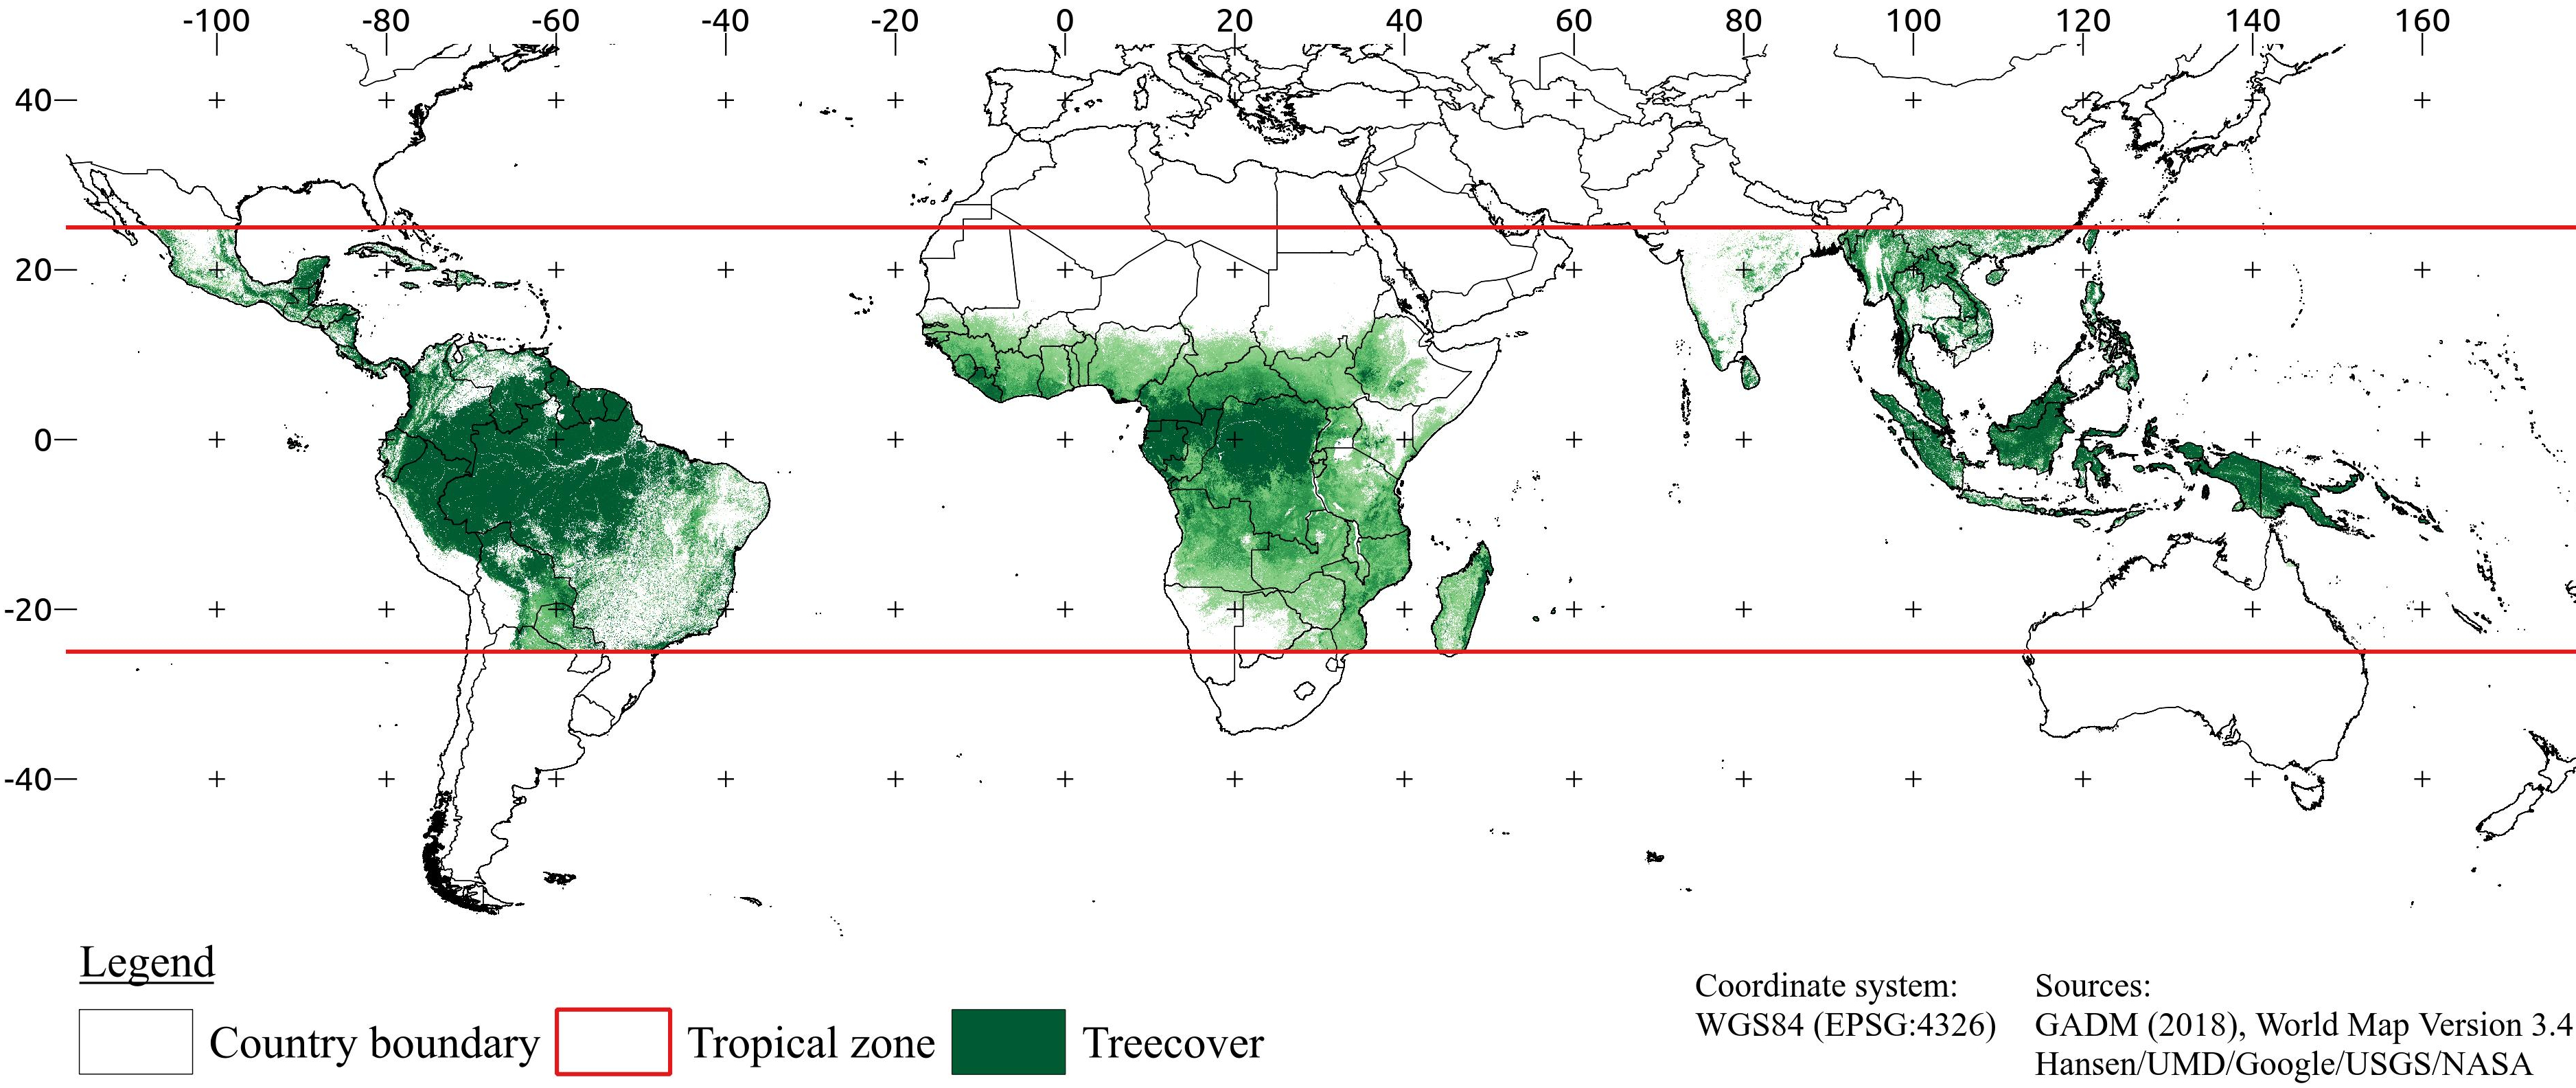
\includegraphics[scale=0.97]{img/intro_overview_frameless}
%		\caption[Tropical zone]{Geographic tropical zone framed red and the tropical forest}
%		\label{fig:tropicalzone}
%	\end{figure}
%	\begin{figure}[ht]
%		\centering
%		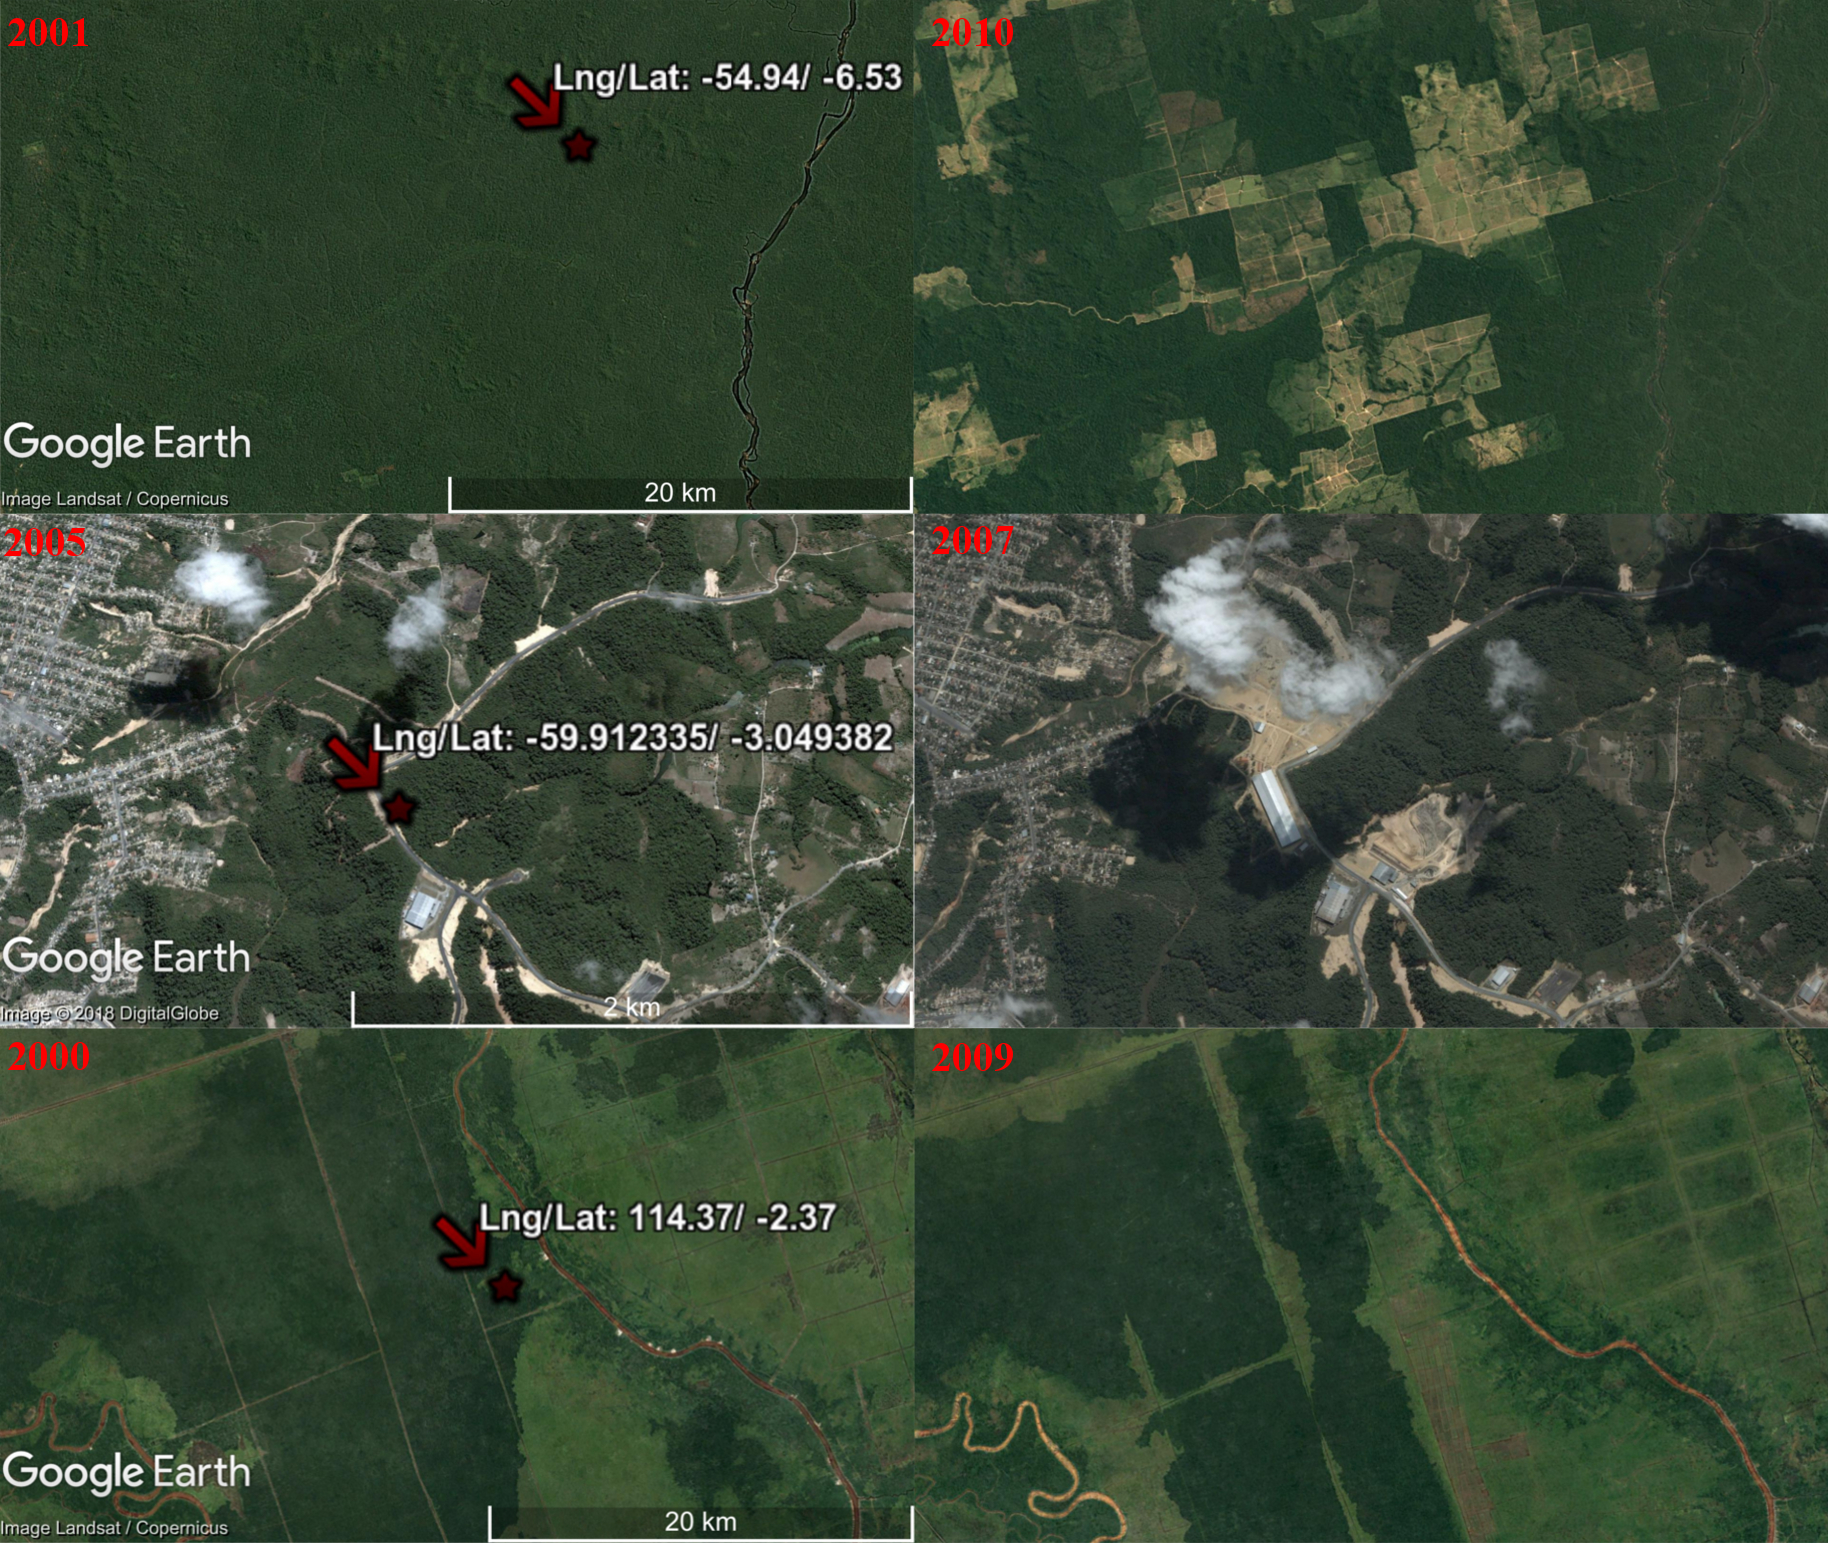
\includegraphics[scale=0.6]{img/deforestation_examples}
%		\caption[Deforestation examples]{Upper Brazil agriculture, middle Brazil urbanization, lower Indonesia large scale palm oil plantations}
%		\label{fig:deforestationexamples}
%	\end{figure}